%\documentclass[12pt,a4paper]{report}
%
%\usepackage[utf8]{inputenc}
%\usepackage[english]{babel}
%\usepackage{amsmath}
%\usepackage{amsfonts}
%\usepackage{amssymb}
%\usepackage{graphicx}
%\usepackage{eurosym}
%\usepackage[left=2cm,right=2cm,top=2cm,bottom=2cm]{geometry}
%\usepackage{wrapfig}
%\usepackage{mathdots}
%\usepackage{caption}
%\usepackage{cite}
%\usepackage{mathrsfs}
%\usepackage{float}
%\usepackage{hyperref}
%
%\author{Josep Maria Serra Moncunill}
%\title{Network Layer Protocols}
%\date{\today}
%
%
%\begin{document}
%
%\maketitle
%\tableofcontents
%\listoffigures
%\listoftables
%
%\chapter{Network Layer}

\subsection{Functions of the Network Layer}
The Network layer provides the following functions:
\begin{itemize}
\item \textbf{Routing}: Selects the best path between two nodes in a network, often using itermediate nodes called routers.
\item \textbf{Network fow control}: Routers may indicate a transmitting node to reduce its transmission when the router's buffer becomes full.
\item \textbf{Package fragmentation}: If the message to be transmitted is too large to be transmitted in the Data link layer, the network may split it into several packages in one node, send them independently an reassemble them in another node. Optionally, it can provide error control.
\item \textbf{Logical-physical adress allocation}: Translates the logical adress (or names) of the network nodes into a unique physical adress.
\item \textbf{Message forwarding}: A network may be divided into subnetworks, connected through specialized hosts, called gateways or routers, that forward packets between those subnetworks.
\end{itemize}
\subsection{Protocols}
\paragraph{}The Consultive Comitee for Space Data Systems (CCSDS)\cite{CCSDSOverview} has two standards for using in the Network layer in conjuction with the Space Data Link Layer Protocols recommended by the CCSDS. Those two standards are the Space Packet Protocol (SPP)\cite{SPP} and the Encapsulation Service\cite{ES}. With the Space Packet Protocol, application processes generate and consume Protocol Data Units (PDU). The Encapsulation Service encapsulates PDU of recognized protocols defined in a Space Assigned Number Authority (SANA)\cite{SANA} registry into two types of packets, either Space Packets or Encapsulation Packets. External protocols data units, such as the Internet Protocol datagrams, can be transmitted by CCSDS Space Data Link Protocols, although they cannot be directly encapsulated by the Encapsulation Service, and an intermediate service, such as IP over CCSDS (IPoC)\cite{IPoC}, must be used.
\paragraph{}Figure \ref{fig:CCSDSprotocols}, shows the recommended protocols by the CCSDS for Space Communications. In Figure \ref{fig:CCSDScombinations} those protocols arearranged in some possible combinations. As it can be seen, IP cannot be directly used neither by the protocols in the Data Link layer nor the Encapsulation Service.
\begin{figure}[H]
\begin{center}
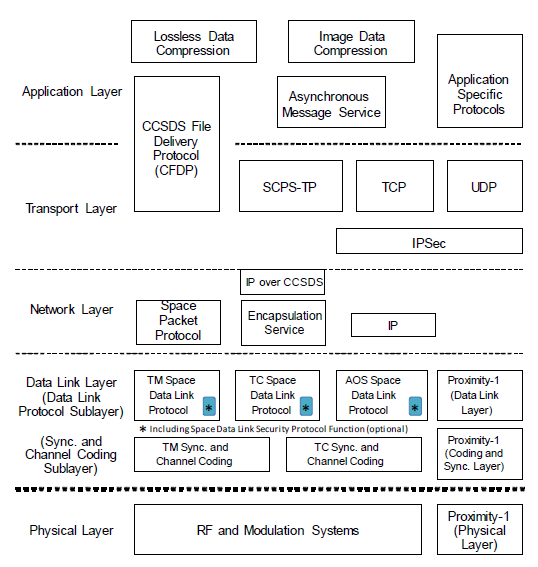
\includegraphics[scale=1]{CCSDSprotocols.PNG}
\caption[CCSDS Recommended Protocols]{Protocols recommended by the CCSDS, classified in their respective OSI layers. Extracted from \cite{CCSDSOverview}.}
\label{fig:CCSDSprotocols}
\end{center}
\end{figure}
\begin{figure}[H]
\begin{center}
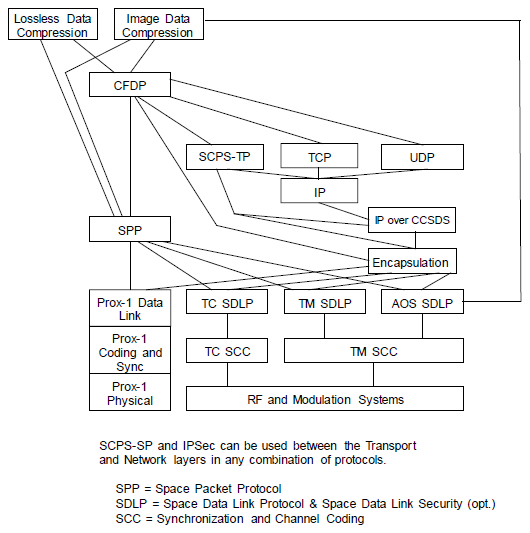
\includegraphics[scale=1]{CCSDScombinations.PNG}
\caption[Combination of CCSDS Recommended Protocols]{Possible Combinations of the CCSDS recommended protocols. Extracted from \cite{CCSDSOverview}.}
\label{fig:CCSDScombinations}
\end{center}
\end{figure}
\paragraph{}Protocols in the Network Layer can be classified according if they are the main protocol (SPP or IP, for example) or they provide additional features so that the main protocol can work efficiently. An example of the latter are routing protocols, and also for IP, IPoC and Encapsulation Service.
\paragraph{}In the following pages, a brief review of distinct protocols on the Network layer will take place. Since CCSDS ecommends using SPP or Encapsulation Service, only SPP and protocols that can be encapsulated by the Encapsulation Service, eiyher directly or indirecly, will be reviewed. The protocols reviewed will be classified according if they are the main protocol, auxiliary protocols, or routing protocols.

\subsubsection{Main protocols}

\subsubsection*{Space Packet Protocol (SPP)\cite{SPP}}
\paragraph{}The Space Packet Protocol (SPP) is a protocol designed to efficiently transfer application data over a network of space links. SPP provides a unidirectional data transfer service from a single source user application to one or more destination user applications through one or more subnetworks. The path from the source user application to the destination user application is called a Logical Data Path (LDP). Every LDP is uniquely identified by a Path Identifier (Path ID). The protocol data unit used by this protocol is the Space Packet. Each Space Packet is defined by a header section and a data section.
\paragraph{}Each LPD is uniquely identified by a Path ID. A Path ID consists of an Application Process Identifier (APID) and an optional APID Qualifier. APID Qualifiers identify the naming domain for an APID. APIDs are unique in a single naming domain. The APID is part of the header of the Space Packet, but the APID Qualifier must be carried by a protocol of an underlying layer.
\paragraph{}The following features are common to the services of the SPP:
\begin{itemize}
\item Pre-configured Services. The user can send or receive data only through a preconfigured LDP established by management.
\item Unidirectional Services. One end of an LDP can send, but not receive, data through the LDP, while the other end can receive, but not send. This means A can send to B through a LPD, but for B to send to A has to use a different LDP
\item Asynchronous Services. There are no predefined timing rules for the transfer of service data units supplied by the service user. The user may request data transfer at any time it desires, but there may be restrictions imposed by the provider on the data generation rate.
\item Unconfirmed Services. The sending user does not receive confirmation from the receiving end that data has been received.
\item Incomplete Services. The services do not guarantee completeness, nor do they provide a retransmission mechanism.
\item Non–sequence Preserving Services. The sequence of service data units supplied by the sending user may not be preserved through the LDP.
\end{itemize}
\paragraph{}The following services are assumed from the underlying layers:
\begin{itemize}
\item Adressing and routing capabilities for establishing LDPs
\item Capability for associating an APID Qualifier for each Space Packet.
\end{itemize}
\paragraph{}The structure of a Space Packet consists of a Packet Primary Header, and a Packet Data Field, which can contain an optional Secondary Header. Figure \ref{fig:SPPheader} shows the structure of the SPP primary header:
\begin{figure}[H]
\begin{center}
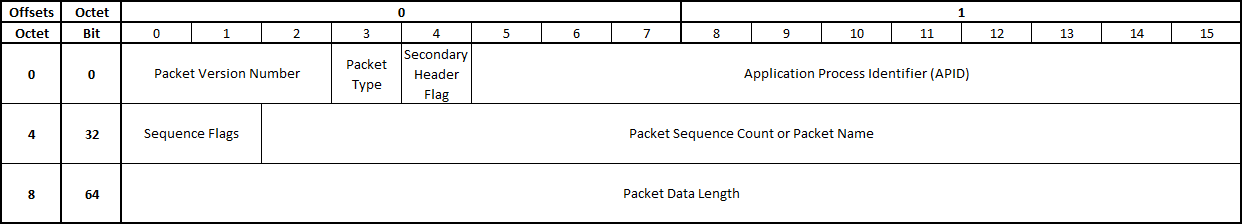
\includegraphics[scale=0.5]{SPP_header.PNG}
\caption[SPP header]{Example of a header for an SPP Space Packet.}
\label{fig:SPPheader}
\end{center}
\end{figure}

\subsubsection*{Internet Protocol version 4 (IPv4)\cite{IP}}
\paragraph{}The Internet Protocol version 4 (IPv4) is the fourth version of the Internet Protocol (IP). It is one of the core protocols of standards-based internetworking methods in the Internet. Despite the ongoing deployment of a successor protocol (IPv6), the IPv4 still routes most of the Internet traffic. IPv4 is a conectionless protocol and does not guarantee delivery, nor does it assure proper sequencing or avoidance of duplicate delivery. These aspects are adressed by a transport layer protocol.
\paragraph{}One of the features of IPv4 are adresses. Network adresses are the identification number of any device that is part of a network. IPv4 uses 32-bit (4 byte) adresses. Therefore, the adress space is limited to 4294967296 ($2^{32}$) adresses. A IPv4 adress is usually represented in two ways: in binary notation, where each group of 8 bits is separated by a dot, or in decimal notation, where each 8-bit binary number is translated to decimal, as it can be seen in Table \ref{table:IPadress}.
\begin{table}[H]
\begin{center}
\begin{tabular}{|l|c|}
\hline 
IP adress & 10101100000100001111111000000001 \\ 
\hline 
Dot-binary notation & 10101100.00010000.11111110.00000001 \\ 
\hline 
Dot-decimal notation & 172.16.254.1 \\ 
\hline
\end{tabular}
\end{center}
\caption[IP adress notation]{IP adress notation in dot-decimal and dot-binary.}
\label{table:IPadress}
\end{table}
\paragraph{}Packets in the IPv4 consist of a header section and a data section. There is no footer at the end of the data section since the protocols in the data link layer and the transport layer provide error correction controls. Headers in a IPv4 packet contain 14 fields, one of them being optional. The fields are packed with the most significant byte first, and the most significant bit is also the first. Headers have a lenght between 20 and 60 bytes. The data section comes after the header, and its format depends on the protocol used (for example, ICMP, IGMP, TCP, etc.). FIgure \ref{fig:IPv4header} shows the structure of a IPv4 header.
\begin{figure}[H]
\begin{center}
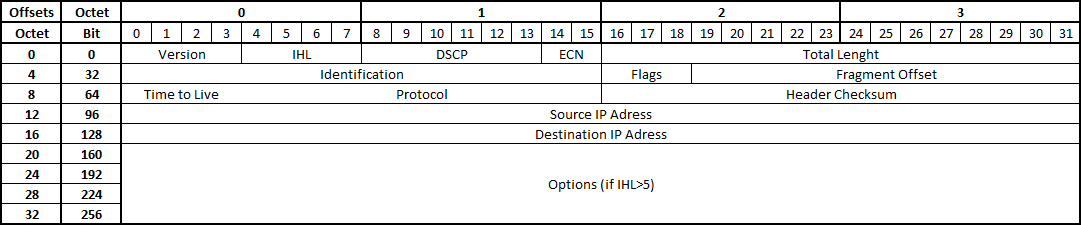
\includegraphics[scale=0.6]{IPv4_header.PNG}
\caption[IPv4 header]{Example of a header for an IPv4 packet. In this case, it has a lenght of 36 bytes.}
\label{fig:IPv4header}
\end{center}
\end{figure}
\paragraph{}IPv4 provides fragmentation of packets. If size of the packet is bigger than the maximum transmission unit (MTU) of the destination, and the message allow fragmentation (the option of Do not Fragment in the header of the packet is set to 0) the transmitting router will divide the packet in fragments smaller than the MTU.

\subsubsection*{Internet Protocol version 6 (IPv6)\cite{IPv6}}
\paragraph{}The Internet Protocol version 6 (IPv6) is the most recent version of the Internet Protocol, developed to solve the problem of the exhaustion of IP adresses of the IPv4. IPv6 is intended to replace IPv4. The new features of the IPv6 compared of those of the IPv4 are the following:
\begin{itemize}
	\item Larger adress space: The length of IPv6 adresses is 128 bits, which is four times the length of IPv4 adresses. It offers a capacity of $2^{128}$ adresses.
	\item Multicasting: IPv6 acomplishes multicasting without using other protocols (such as IGMP for IPv4)
	\item Stateless address autoconfiguration (SLAAC): IPv6 hosts can configure themselves automatically when they are connected to a IPv6 network using the Neighbor Discovery Protocol via Internet Control Message Protocol version 6 (ICMPv6) router discovery messages. When a host is connectes for the first time, it sends a link-local router solicitation multicast request for its configuration parameters. Then, routers respond to the request with a router advertisement packet that contains Internet Layer configuration parameters.
	\item Network-layer security: Internet Protocol Security was developed for IPv6 before it was adapted for IPv4.
	\item Simplified processing by routers: Packet headers and the process of packet forwarding have been simplified, so packet processing by routers is more efficient. Headers now have a fixed length of 40 bytes, and may have an optional section aimed for options between the header section and the data section. Figure \ref{fig:IPv6header} shows the structure of a IPv6 header. IPv6 routers do not perform fragmentation.
	\item Mobility: Mobile IPv6 avoids triangular routing (unlike IPv4) and is as efficient as native IPv6.
	\item Options extensibility: IPv6 headers have astructure capable of extending the protocol in the future without affecting the core packet structure.
	\item Jumbograms: IPv4 limits packets to (2 power 16) - 1 octets per payload. A IPv6 node can handle packets of (2 power 32) - 1 octets (called jumbograms).
\end{itemize}
\begin{figure}[H]
\begin{center}
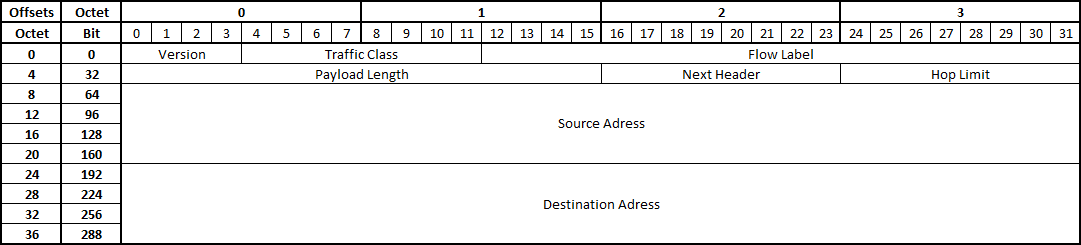
\includegraphics[scale=0.6]{IPv6_header.PNG}
\caption[IPv6 header]{Example of a header for an IPv6 packet.}
\label{fig:IPv6header}
\end{center}
\end{figure}

\subsubsection{Auxiliary protocols}

\subsubsection*{Encapsulation service\cite{ES}}
\paragraph{}The Encapsulation Service is a service used to transfer data units that can not be directly transferred by the CCSDS Space Data Link Protocols. In order to be directly transferred by a Space Data Link Protocol, a data unit must have a Packet Version Number authorized by the CCSDS (a list of PVN authorized by CCSDS is contained in \cite{SANAPVN}). With the Encapsulation Service, data units that do not have an authorized VPN can be transmitted with Space Data Link Protocols. The data unit to be transmitted must be of an integral number of octets.
\paragraph{}A user of the Encapsulation Service is identified by the combination of the following:
\begin{itemize}
\item A Packet Version Number (PVN) that indicates whether Space Packets (PVN=1) or Encapsulation Packets (PVN=8) are used for encapsulation,
\item An Encapsulated Protocol Identifier (EPI), whichis either:
\begin{itemize}
\item An Application Process Identifier (APID) defined in reference (if Space Packets are used).
\item a Protocol ID defined in section 4 of this document (if Encapsulation Packets are used).
\end{itemize}
\end{itemize}
\paragraph{}The APIDs used by the Encapsulation Service must be registered as ‘reserved APIDs’ in \cite{SANAAPID}. The Protocol IDs used by the Encapsulation Service must be registered as ‘defined Protocol IDs’ in \cite{SANAPID}.
\paragraph{}If the Data Unit is encapsulated in a Space Packet, the header format of the Space Packet is the same as the one used by Space Packet Protocol, only that the values of the parameters are restricted to some values. On the other hand, if the Data Unit is encapsulated in a Encapsulation Packet, a different header format will be used. This header have a length of 1-8 octets, and for the case of 8 octet it can be shown in Figure \ref{fig:ESheader}
\begin{figure}[H]
\begin{center}
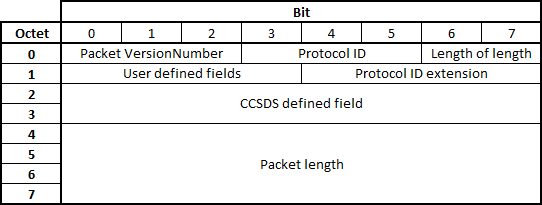
\includegraphics[scale=1]{ES_header.PNG}
\caption[Encapsulation header]{Example of a header for an Encapsulation Packet of maximum length. Some parameters may vary its length in other cases.}
\label{fig:ESheader}
\end{center}
\end{figure}

\subsubsection*{IP over CCSDS (IPoC)\cite{IPoC}}
\paragraph{}The IP over CCSDS is used to transfer IP Data Units over CCSDS Space Data Link Protocols. IP Data Units are encapsulated in Encapsulation Packets and sent through Space Data Link Protocols. IPoC uses the CCSDS Internet Protocol
Extension (IPE) convention in conjunction with the CCSDS Encapsulation Service. The IPE convention is used to add IPE octecs at the beginning of a IP Data Unit, encapsulate the result in an Encapsulation Packet, and transmit it with a CCSDS Space Data Link Protocol. It is used because not all protocols that use an IP datagram have a Protocl ID used by the Encapsulation Packet.
\paragraph{}IPoC adds a header at the beginning of the IP Data Unit, called IPE header. The sum of the IP Data Unit and the IPE header is the Data Unit used by the Encapsulation Service. In other words, for the Encapsulation Service, the IPE header and the IP Data Unit are a whole.
\paragraph{}The structure of the IPE header will be the following. It must be of a length of an integral number of octets, with a minumum length of 1 octet. Each octet will be divided into two parts: the first seven bits (bits 0-6), and the least significant bit (LSB, bit 7). If more octets are added, the LSB of all octets except the last octet are set to '0'. The value of the IPE header is the decimal value of all the octets. The value of the IPE header must be one of the possible values in \cite{SANAIPE}.

\subsubsection*{Internet Control Message Protocol (ICMP)\cite{ICMP}}
\paragraph{}The Internet Control Message Protocol (ICMP) is one of the main protocols of the TCP/IP protocol suite. It is used to send error messages to the source IP of the data packet. It is assigned IP protocol number 1. ICMP messages are typically used for diagnostic, control purposes or generated in response to errors in IP operations. They are processed differently than normal IP proceessing.
\paragraph{}There are many types of control messages that the ICMP can send:
\begin{itemize}
\item Souce quench: Used to request the sender to decrease the rate of messages sent to a router.
\item Redirect: Used to request the sender to send the data to another router.
\item Time exceeded: Used by a gateway to inform the sender of a discarded datagram due to the time to life field reaching zero. It is also used to inform the sender that a fragment of a message has not been reassembled within the time limit
\item Timestamp: Used for time syncronization. The sender sends the timestamp it last touched the packet (in miliseconds since midnight)
\item Timestamp reply: Used to reply a timestamp. The reciever of the timestamp message replies the sender with the original timestamp, the timestamp when the message was recieved, and the timestamp when the reply was sent.
\item Adress mask request: Used by a host to obtain the subnet mask of a router
\item Adress mask reply: Used to reply the adress mass request returning the subnet mask.
\item Destination unreachable: Used by the host or its inbound gateway to inform the client that the destination is unreachable.
\end{itemize}

\subsubsection*{Internet Control Message Protocol version 6 (ICMPv6)\cite{ICMPv6}}
\paragraph{}The Internet Control Message Protocol version 6 (ICMPv6) is the implementation of the ICMP for IPv6. Several extensions have been published that define new types of ICMPv6 messages, as well as new options for existing message types. One of those is the Neighbor Discovery Protocol (NDP), a node discovery protocol for IPv6 that replacesand enhances the features of the Address Resolution Protocol (ARP). Secure Neighbor Discovery (SEND) is, respectively, an extension of NDP with extra security. Multicast Router Discovery (MRD) allows discovery of multicast routers.

\subsubsection*{Internet Group Management Protocol (IGMP)\cite{IGMP}}
\paragraph{}The Internet Group Management Protocol (IGMP) is used by hosts and adjacent routers on IPv4 networks to establish multicast group memberships. It is a part of IP multicast, and it is used in one-to-many networking applications such as online streaming video. IGMP operates between the client computer and a local multicast router. IGMP messages are carried in bare IP packets with protocol number 2.

\subsubsection*{Internet Protocol Security (IPsec)\cite{IPsec}}
\paragraph{}The Internet Protocol Security (IPsec) is a protocol suite for secure Internet Protocol (IP) communications. It authenticates and encrypts each IP packet of a communication session. IPSec includes protocols for establishing mutual authentication between agents at the beginning of the session and negotiation of cryptographic keys to be used during the session. IPsec can be used in protecting data flows between a pair of hosts (host-to-host), between a pair of security gateways (network-to-network), or between a security gateway and a host (network-to-host). It supports network-level peer authentication, data origin authentication, data integrity, data confidentiality (encryption), and replay protection.
\paragraph{}IPsec uses the following protocols to perform various functions;
\begin{itemize}
\item Authentication Headers (AH): Provides connectionless data integrity and data origin authentication for IP datagrams, and provides protection against replay attacks.
\item Encapsulating Security Payloads (ESP): Provide confidentiality, data-origin authentication, connectionless integrity, an anti-replay service, and limited traffic-flow confidentiality.
\item Security Associations (SA): Provides the bundle of algorithms and data that provide the parameters necessary for AH and ESP operations.
\end{itemize}

\subsubsection*{Protocol Independent Multicast (PIM)\cite{PIMSM}\cite{PIMDM}}
\paragraph{}The Protocol Independent Multicast (PIM) is a family of multicast routing protocols for Internet Protocol (IP) networks that provide one-to-many and many-to-many distribution of data. PIM does not include its own topology discovery mechanism, but instead uses routing information supplied by other routing protocols.
\paragraph{}There are four variants of PIM:
\begin{itemize}
\item PIM Sparse Mode (PIM-SM): It builds unidirectional shared trees rooted at a rendezvous point (RP) per group, and optionally creates shortest-path trees per source. It is called sparse-mode because it is suitable for groups where low percentage of the nodes will subscribe to the multicast session.
\item PIM Dense Mode (PIM-DM): It uses dense multicast routing. It builds shortest-path trees by flooding multicast traffic domain wide, and then pruning back branches of the tree where no receivers are present. Dense mode is ideal for groups where many of the nodes will subscribe to receive the multicast packets.
\item Bidirectional PIM: It builds shared bi-directional trees. It never builds a shortest path tree, so may have longer end-to-end delays than PIM-SM.
\item PIM Source-Specific Multicast (PIM-SSM): It builds trees that are rooted in just one source, offering a more secure model for a limited amount of applications (mostly broadcasting of content). In SSM, an IP datagram is transmitted by a source S to an SSM destination address G, and receivers can receive this datagram by subscribing to channel (S,G).
\end{itemize}

\subsubsection{Routing protocols}

\subsubsection*{Enhanced Interior Gateway Routing Protocol (EIGRP)\cite{EIGRP}}
\paragraph{}The Enhanced Interior Gateway Routing Protocol (EIGRP) is a routing protocol used on a computer networks for automating routing decisions and configuration. This protocol was designed by Cisco Systems and it was only avaiable for Cisco routers. In 2003, partial functionality of EIGRT was converted to an open standard and in 2016 was published with informational status. EIGRP is used on a router to share routes with other routers in the same autonomous system.
\paragraph{}All routers contain a routing table that lists the routes to network destinations. If a router cannot find a valid path to the destination, the traffic is discarded. EIGRP is a dynamic routing protocol, which means that routers automatically exchange information about routes and, therefore, the administrator does not have to change the routing table manually. Besides the routing table, routers adittionlly have two more tables.
\begin{itemize}
\item Neighbour table. It stores the IP adress of the routers that have a direct connection with this router. If a router is connectedto another with an intermediate router, it will not be recorded in this table.
\item Topology table. It keeps record of routes that has learned from neightbouring router tables, and also records the distance (number of intermediate routers) of each route, the feasible successor and the successors (other routes that have the same destination and are loop free). Routes in this table are either labelled as "passive" or "active". Passive means that EIGRP  has determined the path for the specific route and has finished processing. Active means that EIGRP is still trying to calculate the best path for the specific route. The router dones not use the routes in this table. A route in this table will be inserted in the routing talbe when is marked as passive, is not a feasible successor and does not have a higher distance than an equivalent path
\end{itemize}
\paragraph{}If there is a change in the network (a link fails, or a router is disconnected), the path becomes unavaiable, and is removed from the routing table. The routing table of a router will be updated, and only the changes since the previous update will be transmitted to the neightbouring routers. The information about the changes in the routing table is not transmitted periodically, but only when a change actually occurs.
\paragraph{}EIGRP supports the following features:
\begin{itemize}
\item Support for Classless Inter-Domain Routing (CIDR) and variable length subnet masking. Routes are not summarized at the classful network boundary unless auto summary is enabled.
\item Support for load balancing on parallel links between sites.
\item The ability to use different authentication passwords at different times.
\item MD5 authentication between two routers.
\item Sends topology changes, rather than sending the entire routing table when a route is changed.
\item Periodically checks if a route is available and propagates routing changes to neighboring routers if any changes have occurred.
\item Runs separate routing processes for Internet Protocol (IP), IPv6, IPX and AppleTalk through the use of protocol-dependent modules (PDMs).
\end{itemize}
\paragraph{}EIGRP does not operate using the Transmission Control Protocol (TCP) or the User Datagram Protocol (UDP). This means that EIGRP does not use a port number to identify traffic. Rather, EIGRP is designed to work on top of layer 3. Since EIGRP does not use TCP for communication, it implements Cisco's Reliable Transport Protocol (RTP) to ensure that EIGRP router updates are delivered to all neighbors completely.

\subsubsection*{Open Shortest Path First (OSPF)\cite{OSPFv2}\cite{OSPFIPv6}}
\paragraph{}The Open Shortest Path First (OSPF) is a routing protocol for Internet Protocol (IP) networks that operates in a single autonomous system. OSPF version 2 is designed for IPv4, while OSPF version 3 is designed for IPv6. It works by gathering link state information from available routers and constructing a topology map of the network. The topology is presented as a routing table to the Internet layer which routes packets based solely on their destination IP address. OSPF detects changes in the topology, such as link failures, and creates a new loop-free routing structure. It computes the shortest-path tree for each route using a method based on Dijkstra's algorithm. OSPF does not use a transport protocol, such as UDP or TCP, but encapsulates its data directly in IP packets with protocol number 89. It implements its own transport layer error detection and correction functions. OSPF uses multicast addressing for distributing route information within a broadcast domain.
\paragraph{}OSPF supports complex networks with multiple routers, including backup routers, to balance traffic load on multiple links to other subnets. Routers form adjacencies when they have detected each other. This detection is initiated when a router identifies itself in a Hello protocol packet. Upon acknowledgment, this establishes a two-way state and the most basic relationship. The routers in an Ethernet or Frame Relay network select a Designated Router (DR) and a Backup Designated Router (BDR) which act as a hub to reduce traffic between routers. OSPF establishes and maintains neighbor relationships for exchanging routing updates with other routers. The neighbor relationship table is called an adjacency database. Two OSPF routers are neighbors if they are members of the same subnet and share the same area ID, subnet mask, timers and authentication. OSPF adjacencies are formed between selected neighbors and allow them to exchange routing information. Two routers become adjacent if at least one of them is Designated Router or Backup Designated Router (on multiaccess type networks), or they are interconnected by a point-to-point or point-to-multipoint network type.
\paragraph{}OSPF does not carry data via a transport protocol. Instead, OSPF forms IP datagrams directly, packaging them using protocol number 89 for the IP Protocol field. OSPF defines five different message types, for various types of communication:
\begin{itemize}
\item Hello: It is used to allow a router to discover other adjacent routers on its local links and networks. The messages establish adjacencies between neighboring devices. uring normal operation, routers send hello messages to their neighbors at regular intervals. If a router stops receiving hello messages from a neighbor, after a set period the router will assume the neighbor has gone down.
\item Database Description: It contain descriptions of the topology of the autonomous system or area.  They convey the contents of the link-state database (LSDB) for the area from one router to another. Communicating a large LSDB may require several messages to be sent.
\item Link State Request: These messages are used by one router to request updated information about a portion of the LSDB from another router. The message specifies exactly which link about which the requesting device wants more current information.
\item Link State Update: These messages contain updated information about the state of certain links on the LSDB. They are sent in response to a Link State Request message, and also broadcast or multicast by routers on a regular basis. Their contents are used to update the information in the LSDBs of routers that receive them.
\item Link State Acknowledgment: These messages provide reliability to the link-state exchange process, by explicitly acknowledging receipt of a Link State Update message.
\end{itemize}

\subsubsection*{Routing Information Protocol (RIP)\cite{RIPv2}\cite{RIPng}}
\paragraph{}The Routing Information Protocol (RIP) is a routing protocol. It uses a hop count to establish the distance between two routers and, in order to prevent loops, establishes 15 as the limit number of hops in a route. If the number of hops is 16, the distance between the two routers is considered infinite. Each router has a routing table with all the routes to each possible destination, and the number of hops to get there. There are 3 versions of RIP: RIPv1, which is the original, RIPv2, which is an updated version of RIPv2, and RIPng, which is the new generation of RIP compatible with IPv6.
\paragraph{}The operating principle of the RIP is the following: When a RIP router comes online, it sends a broadcast message to all of its RIP enabled interfaces. All the neighbouring routers that receive the Request message respond back with the Response Message containing their Routing table. The Response Message is also gratuitously sent when the Update timer expires (by deffect, 30 seconds). On receiving the Routing table, the router processes each entry of the routing table as per the following rules:
\begin{itemize}
\item{} If there are no route entries matching the one received then the route entry is added to the routing table automatically, along with the information about the router from which it received the routing table.
\item{} If there are matching entries but the hop count metric is lower than the one already in its routing table, then the routing table is updated with the new route.
\item{} If there are matching entries but the hop count metric is higher than the one already in its routing table, then the routing entry is updated with hop count of 16 (infinite hop). The packets are still forwarded to the old route. A Holddown timer is started and all the updates for that route from other routers are ignored. If after the Hold-down timer (per deffect 180 seconds) expires and still the router is advertising with the same higher hop count then the value is updated into its routing table. Only after the timer expires, the updates from other routers are accepted for that route.
\end{itemize}
\paragraph{}If the Invalid timer (per deffect 180 seconds) expires and a routing entry has not been updated, the hop counter of that route will be set to 16, marking the route as invalid. Then, if the Flush timer (per deffect 240 seconds) expires, the invalid route entry will be removed

\subsection{Protocol Selection}

\subsubsection{Choice of the main protocol}
\paragraph{}The choice of the main protocol will be between SPP, IPv4 and IPv6. Tho make the choice, it is important to take into account that the Astrea constellation is a network that can be of more than two hundred satelites, which will communicate point-to-point. Each node can be the source ,the destination or an intermediate node of a communication route.
\paragraph{}SPP has the advantage of being designed to work easily with the protocols of the adjacent layers, while IP needs IP over CCSDS and Encapsulation Service. However, SPP requires a parametre called Path ID, which is the identifier of a Logical Data Path. Since each satellite of Astrea constellation can be the source or the destination of a data path, this means that for a network of 200 nodes, there are 200x199=39800 possible routes. The parameter to indicate the Path ID has a length of 11 bits, which can identify 2048 different routes, which is not enough. Another issue to take into account is that since the ground station nodes of the constellation are moving respect the satellite nodes, their relative position changes and, therefore, paths also change. If the path associated to a Path ID changes during a transmission, or if is not updated for all nodes at the time of the transmission, errors can occur. This does not happen with IP, since instead of Path ID it uses the IP adress of the source and destination node. For this reason, SPP is discarded.
\paragraph{}The main differences between IPv4 and IPv6 are the header of the datagram and the IP adresses of the nodes. Since our  network is private and it is not intended to be connected to the Internet, nodes can have an arbitrary IP adress assigned. For this reason, IPv4 adresses are better, since they are shorter than IPv6 adresses. The size of the header would also be smaller in IPv4 than IPv6. However, for long datagrams, the extra length of IPv6 headers is irrelevant. Another difference is that IPv6 datagrams require less processing power, however, since the processing power is very small compared to the power required by the antennas this factor also has little importance in terms of power. However, it is important in terms of time, since less processing means less time to process. Other features of IPv6 that, in Astrea network, do not privide benefits are the multicast and mobility features, which the network ill not have. Additionally, due to the changing nature of the constellation, jumbograms will not be used because a packet so long may be interrumted when the path changes.
\paragraph{}The real benefits of IPv6 over IPv4 is that there are less additional protocols compared to IPv4 to perform the same features, since ICMPv6 provide the features of ICMP, ARP and IGMP, and some features of IPv6 itself and its additional protocols have been eliminated since they were already performed by other layer protocols and were redundant. All of this helps to reduce the time required to process the data and this, in long paths, is a significant factor.
\paragraph{}If reliable adjacent layer protocols are provided, IPv6 is the best option, due to less processing in routers and more simple additional protocols. Additionally, IPv6 is progressively replacing IPv4 and, therefore, using IPv6 has no risk of being obsolete.

\subsubsection{Choice of routing protocol}
\paragraph{}The choice of the routing protocol will be between EIGRP, OSPF and RIP.
\paragraph{}EIGRP is a protocol compatible with either IPv4 and IPv6. Contrary to other protocols, it only sends topology changes instead of the whole routing table, allowing for less data transmitted. It also contains more information about routes than other routing protocols, and provides authentication processes.
\paragraph{}RIP is a protocol that, compared to EIGRP and OSPF, has the drawback that its time to converge and its scalability are poor. Additionally, RIP uses the User Datagram Protocol (UDP) as its transport protocol. On the other, it is easier to configure than other protocols.
\paragraph{}OSPF is a protocol also compatible with IPv4 and IPv6. Unlike EIGRP, each router exchanges its adjacency links with adjacent routers and then, each router creates its own map of the network and, using this map, each router creates its own routing table. However, it has mechanisms to ensure that thare are not loops in the network.
\paragraph{}Taking into account that nodes in the Astrea network have an order of magnitude of 200 and is continously changing the data paths. Also, since Astrea is a network where a node can be the beginning or the end of a communication, this means that for a given node there has to be a route to every other node in the network, and for a network of 200 nodes, there are 199 possible routes for the 200 nodes, which is a total of 39800 different entries in the routing table only for the satellite nodes. Since RIP has longer time to converge compared to other protocols, and due to the huge size of the routing table, RIP is discarded.
\paragraph{}EIGRP does not have this problem because it does not transmit the whole routing table, but only the changes. Although the network is continously moving, the paths between the satellite nodes remain the same. The problem happens with the ground nodes, which are continouslly changing its position respect the satellite nodes due to Earth's rotation. And since each satellite node can communicate with every ground station, the number of entries in the routing table that will be updated for a network of 200 satellite nodes and 5 ground stations is 200x5, which is 1000 entries that will be updated frequently. Since OSPF does not transmit the routing table but only the adjacencies, only 205 entries will be transmitted. This reduces the time to share the updated information to the whole network. For this reason, OSPF is chosen.

\subsubsection{Choice of complementary protocols}
\paragraph{}The choice of which protocols include will depend on the main protocol of the network layer and the degree of services featured by the communication process.
\paragraph{}Since IPv6 has been chosen, IP over CCSDS and Encapsulation Service are necessary. Additionally, ICMPv6 greatly expand the features of IPv6 such as flow control. Security features are already provided in the Data Link layer and, therefore, IPsec is not necessary. Also, no multicast features are required, so no multicast protocols will not be used.

\subsubsection{Conclusion}
\paragraph{}It has been decided that IPv6 will be the network layer protocol, complemented with IPoC, Encapsulation Service and ICMPv6, and with OSPF as the routing protocol.

\subsection{Final structure}
\paragraph{}As the protocols have already been chosen, it is time to establish how will be the headers of the different protocols.
\paragraph{}The IPv6 header will depend greatly on the protocol of the upper layers, or the auxiliar protocol (OSPF, ICMPv6). The main parameters of the IPv6 header, that can be seen in Figure \ref{fig:IPv6header}, are the following:
\begin{itemize}
\item \textbf{Version} Current version of IP, which for IPv6 is 6 (bit sequence 0110).
\item \textbf{Traffic Class}. The bits of this field hold two values. The 6 most-significant bits are used for differentiated services, which is used to classify packets. The remaining two bits are used for ECN; priority values subdivide into ranges: traffic where the source provides congestion control and non-congestion control traffic.
\item \textbf{Flow Label}. The flow label when set to a non-zero value now serves as a hint to routers and switches with multiple outbound paths that these packets should stay on the same path so that they will not be reordered.
\item \textbf{Payload Length}. The size of the payload in octets, including any extension headers. The length is set to zero when a Hop-by-Hop extension header carries a Jumbo Payload option.
\item \textbf{Next Header}. Specifies the type of the next header. This field usually specifies the transport layer protocol used by a packet's payload. When extension headers are present in the packet this field indicates which extension header follows. The values are shared with those used for the IPv4 protocol field, as both fields have the same function (see List of IP protocol numbers in \cite{IANAPN}).
\item \textbf{Hop Limit}. This value is decremented by one at each intermediate node visited by the packet. When the counter reaches 0 the packet is discarded.
\item \textbf{Source Address}. The IPv6 address of the sending node.
\item \textbf{Destination Address}. The IPv6 address of the destination node.
\end{itemize}
\paragraph{}It has been stated that, since Astrea network is a private network that will not be connected to the Internet, IP adresses will be arbitrary assigned to the nodes of the network.
\paragraph{}For the IPoC heaver, the value for IPv6 datagrams is 87, so the header of OPoC will be 01010111
\paragraph{}For the Encapsulation Service, depending of the length of the data unit transmitted, the header will very. For data units up to 65531 octets, the Encapsulation Service header will be the following: 11101010-00000000-XXXXXXXX-XXXXXXXX, where XXXXXXXX-XXXXXXXX is the binary number of the total length of the Encapsulation Packet, including the Encapsilation Packet header.